\chapter{Temporary Chapter(Overall Design)}
An attempt at giving an overall design for the program, and its different parts.
\section{Design Goals}
\begin{itemize}
	\item Its better with a smart data structure surrounded by dumb code than a dumb data structure and smart code!!
	\item Clear and clean separation of the front-end and the back-end so in the future other parsers can be used to generate dissectors
	\item Try to be pythonic, follow PEP8 and PEP20.
	\item Now is better than never. Don't be afraid to write stupid or ugly code, we can always fix it later.
	\item The first version is never perfect, so don't wait until its perfect before you commit. Commit often!
\end{itemize}

\section{Architecture}
Figure \ref{fig:archdesign}

\begin{figure}[!ht]
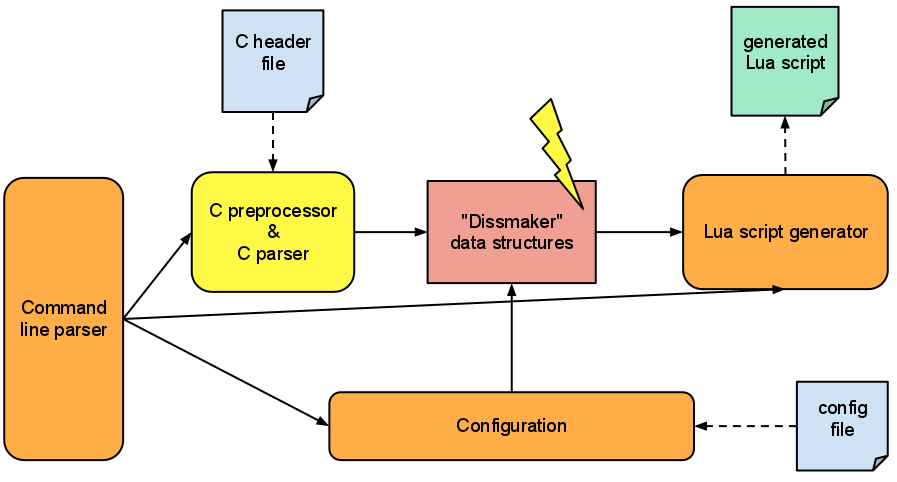
\includegraphics[width=\textwidth]{./planning/img/overall_design.png}
\caption{Overall Architecture}
\label{fig:archdesign}
\end{figure}

\section{Overall design}
\begin{itemize}
	\item The program is split into several parts.
	\item The part which the user runs, should accept arguments which specifies which files to parse and config files to use. It should ask the configuration to parse config files, then ask the front-end to parse c files, and finally ask the back-end to generate Wireshark dissectors.
	\item Configuration should parse config files and feed information to the other parts, or they should request informations when they need it.
	\item Front-end C parser should parse C files and look for struct definitions, which they will fill into some data-structures that the back-end will use.
	\item The data structures should store the information the back-end needs to generate Wireshark dissectors.
	\item The back end should use information in the data structures to generate Wireshark dissectors written in Lua.
\end{itemize}

\section{Command line arguments}
\begin{itemize}
	\item  Should probably use argparse module from python standard library.
	\item Needs to parse commands given when the program is started, and supply them to other parts of the program who needs them.
	\item It must fulfill the following requirements:
	\begin{itemize}
		\item FR7-A Command line shall support parameters for c-header file
		\item FR7-B Command line shall support for configuration file
		\item FR7-C Command line shall support batch mode of c-header and configuration file
		\item This simply means it should accept arguments for 0, 1, or more C code files, and/or 0 or 1 configuration file.
	\end{itemize}
	\item It would be useful if it could also support:
	\begin{itemize}
        		\item -v or -verbose: which should print information about AST tree etc.
        		\item -d or -debug: which should print which steps are happening in the process
        		\item -nocpp: option to disable the C preprocessor
        		\item option(s) to specify which folders to include in the C preprocessor step
        		\item option which specifies where the output should be saved
        		\item printing of help/usage information if one gives it no commands or wrong command
	\end{itemize}
\end{itemize}

\section{Configuration}
\begin{itemize}
	\item Parse one (or more?) configuration files which can be used to modify the process of generation dissectors.
	\item Should maybe only modify data structures?
	\item Challenging part is designing how do we support the different scope of configuration: 
	\begin{itemize}
		\item Can refer to a specific named struct
		\item Can refer to a specific C file?
		\item Can refer to all structs
		\item Can refer to a specific type like time\_t
	\end{itemize}
	\item Must fulfill the following requirements: 
	\begin{itemize}
        		\item Must support valid ranges for struct members
        		\item Must support integer members which represent enumerated named value or a bit string
        		\item Must support custom handling of specific data types
        		\item A struct may have a header and/or trailer (other registered protocol). The configuration must support the use of integer members to indicate the number of other structs that will follow in the trailer
	\end{itemize}
\end{itemize}

\section{C parser, front-end}
\begin{itemize}
	\item Use pycparser and PLY libraries for parsing of C files.
	\item Use cpp and fake libc include files, which comes with pycparser, for C preprocessor step as long as possible.
	\item Should accept C header/code files and create an abtract syntax tree, which it then traverses and finds struct defintions and their members.
	\item Should fill in the necessary information into the data structures, so that the dissector generator can create dissectors for the structs.
	\item Must fulfill the following requirements:
	\begin{itemize}
		\item Must be able to read basic C language struct definitions from C header files
		\item Must support the following basic data types: int, float, char and boolean
		\item Must support members of type enums, structs, unions and arrays
    		\item Must support C preprocessor directives and macros: \#include, \#define, \#if, WIN32, \_WIN32, \_WIN64, sparc, \_\_sparc and sun
	\end{itemize}
\end{itemize}

\section{Data structures}
\begin{itemize}
	\item Should be focused on what data is needed to create Wireshark dissectors.
	\item Should support configuration modifying it.
	\item Should be smart, but not magic.
\end{itemize}

\section{Dissector generator, back-end}
\begin{itemize}
	\item Should accept data structures and create Wireshark dissectors written in Lua.
	\item Must fulfill the following requirements: 
	\begin{itemize}
		\item Must be able to generate lua-script for Wireshark dissectors for the binary representation of C structs.
		\item Shall be able to display simple structs and structs within structs
		\item Must support Wiresharks built-in filter and search on attributes
		\item Shall be able to recognize invalid values for a struct member
	\end{itemize}
\end{itemize}

\section{Handle binary input which size and endian depends on platform}
\begin{itemize}
	\item I dont know yet how we will do this
	\item Flags?
\end{itemize}